% plane_wave_limit_restructured.tex
\documentclass[12pt,a4paper]{article}

% ---------- 语言与版面 ----------
\usepackage{xeCJK}          % 中文支持,不显式指定 CJK 字体,xeCJK 会选系统里第一款可用中文字体
\usepackage{fontspec}
\usepackage{geometry}
\geometry{left=2.5cm,right=2.5cm,top=2.8cm,bottom=2.8cm}
\usepackage{graphicx}       % 插图
\usepackage{amsmath,amssymb}
\usepackage{siunitx}        % 单位与数字
\sisetup{detect-all=true}
\usepackage{booktabs}       % 表格
\usepackage{multirow}        % 多行表格
\usepackage{hyperref}       % 超链接
\hypersetup{colorlinks=true, linkcolor=blue, citecolor=blue, urlcolor=blue}

% ---------- 文档信息 ----------
\title{圆柱形波导平面波模型高频局限性分析 \\\\ (以 $D=\SI{29.5}{mm}$ 为例)}
\author{ } % 作者留空或填写
\date{\today}

\begin{document}
\maketitle

\begin{abstract}
本文针对直径 $D=\SI{29.5}{mm}$ 的理想刚性圆柱形波导,系统地分析了一维平面波声学模型在高频应用时的局限性。首先,通过经典声学理论,推导出波导内高阶模态的截止频率计算公式,明确指出首个非平面模态 $(\psi_{11})$ 的理论截止频率约为 \SI{6.9}{kHz}。随后,利用 Python 编程(结合 SciPy 和 Matplotlib 库)实现了多模态计算,对理论结果进行了数值验证,并直观展示了各阶模态在波导横截面上的声压分布。研究结果精确地表明:当声波频率高于 \SI{6.9}{kHz} 时,波导内声场开始呈现显著的三维特性,一维平面波假设不再适用。此结论对于准确进行宽带语音信号分析、声道高频声学特性建模以及声辐射指向性预测等研究具有重要的参考价值,提示在涉及较高频率时必须考虑采用多模态理论或三维数值方法。\par
\vspace{1em}
\textbf{关键词:} 平面波假设;截止频率;高阶模态;贝塞尔函数;圆柱波导;Python数值模拟
\end{abstract}

\tableofcontents
\newpage

%======================================================================
\section{引言}
%======================================================================

\subsection{声道声学建模现状}
对人类语音产生机理的研究中,声道(Vocal Tract)的声学特性是核心环节之一。物理模型,特别是基于简化几何形状的一维模型,因其计算高效、易于理解,在语音合成、音色分析以及发声障碍诊断等领域得到了广泛应用~\cite{bib:Story1996, bib:Fant1960}。这些模型通常将复杂三维的声道简化为一系列变截面声管的串联,并通过面积函数描述其几何形态。

\subsection{平面波假设及其局限}
在传统的声道声学模型中,普遍采用\textbf{一维平面波假设}。该假设认为声波在声道内传播时,其波阵面始终垂直于传播方向(声道轴线),且在任意横截面上声压均匀分布。在此前提下,声道的声学特性仅由其面积函数决定,大大简化了数学处理和计算复杂度。这一模型在较低频率范围(通常认为低于 \SIrange{4}{5}{\kilo\hertz})能够较好地吻合实验观测,足以满足早期语音识别和窄带语音合成的需求。

然而,随着对语音质量(如自然度、可懂度)要求的提高以及宽带语音技术的发展,研究者逐渐认识到高频成分(超过 \SI{5}{\kilo\hertz})对音色感知、辅音清晰度乃至情感表达的重要性~\cite{bib:Monson2014HighFreq, bib:Vampola2015HighFreqSpeech}. 在这些较高频率下,声波波长逐渐缩短,可能与声道横向尺寸处于同一量级。此时,平面波假设的物理基础不再牢固,声场在横截面内可能出现显著变化,即\textbf{高阶模态 (Higher Order Modes, HOMs)} 被激发。这些高阶模态的出现,使得一维模型无法准确描述声波在声道内的传播和辐射特性,从而限制了其在高频研究中的应用。

\subsection{本文工作与创新点}
为精确揭示一维平面波模型在高频段的失效边界,本文以一个具有代表性的固定直径($D=\SI{29.5}{mm}$)的理想刚性圆柱形波导为研究对象——该尺寸与人声道的平均有效直径具有可比性。本文的主要工作包括:
\begin{itemize}
    \item 从三维波动方程出发,详细推导圆柱波导内高阶模态的截止频率公式。
    \item 针对 $D=\SI{29.5}{mm}$ 的具体案例,计算首个及后续几个高阶模态的理论截止频率。
    \item 采用 Python 语言(结合 SciPy 科学计算库)编写数值程序,独立计算各模态的截止频率,并与理论值进行交叉验证。
    \item 利用 Matplotlib 库可视化各模态在波导横截面上的声压分布(模态形状图)。
    \item 结合波长与管道直径的相对关系,讨论平面波假设的有效频率上限。
\end{itemize}
本文的创新点在于,通过理论分析与数值模拟相结合的方式,对特定几何参数下的平面波局限性给予定量、精确的界定,并提供了可复现的计算方法和直观的物理图像,为后续更复杂的声道声学研究(如考虑弯曲、变截面、粘滞热损耗等因素)提供了一个清晰的理论基准。

%======================================================================
\section{圆柱波导声学理论与平面波条件}
%======================================================================

\subsection{参数与符号}
本文所涉及的主要物理量、符号及其典型取值(针对空气介质和特定案例)如表~\ref{tab:param} 所示。

\begin{table}[h!]
    \centering
    \caption{主要物理参数与符号定义}\label{tab:param}
    \begin{tabular}{llc}
        \toprule
        符号 & 定义 & 典型值 / 单位 \\
        \midrule
        $c$     & 空气中声速(本文设 $T=\SI{26.5}{\celsius}$) & $\approx \SI{347.1}{\meter\per\second}$ \\ % Recalculate for T=26.5
        $f$     & 频率 & \si{\hertz} \\
        $\rho$   & 空气密度(标准状况) & $\approx \SI{1.204}{\kilo\gram\per\cubic\meter}$ \\ % at 20C, or specify T
        $\lambda$ & 波长,$\lambda = c/f$ & \si{\meter} \\
        $k$     & 自由场波数,$k = \omega/c = 2\pi/\lambda$ & \si{\radian\per\meter} \\
        $D$     & 波导直径 & \SI{29.5}{\milli\meter} \\
        $R$     & 波导半径,$R = D/2$ & \SI{14.75}{\milli\meter} \\
        $m,n$   & 模态阶数(径向$m$, 角向$n$) & $0,1,2,\dots$ \\
        $\psi_{mn}$ & $(m,n)$ 阶模态函数 & -- \\
        $\mu_{mn}$  & Bessel 函数导数 $J'_n(x)$ 的第 $m$ 个零点 & -- \\
        $f_{c,mn}$ & $(m,n)$ 阶模态的截止频率 & \si{\hertz} \\
        \bottomrule
    \end{tabular}
\end{table}
注:声速 $c$ 由 $c = 331.3 \sqrt{1 + T/273.15}$ 计算,其中 $T$ 为摄氏温度。空气密度 $\rho$ 也会随温度略有变化,但对截止频率计算无直接影响。

\subsection{三维波动方程与亥姆霍兹方程}
在无粘性、均匀的理想流体介质中,小振幅声波的声压 $p(x_1,x_2,x_3,t)$ 满足三维波动方程:
\begin{equation}
    \nabla^{2} p - \frac{1}{c^{2}}\frac{\partial^{2}p}{\partial t^{2}} = 0.
    \label{eq:wave3d}
\end{equation}
对于简谐波 $p(x_1,x_2,x_3,t) = P(x_1,x_2,x_3)e^{j\omega t}$,波动方程转化为亥姆霍兹方程:
\begin{equation}
    \nabla^{2} P + k^2 P = 0, \quad \text{其中 } k = \omega/c \text{ 为自由场波数.}
    \label{eq:helmholtz}
\end{equation}

\subsection{圆柱波导中的可分离解与特征方程}
在圆柱坐标 $(r,\theta,z)$ 下,设声压的复振幅形式为 $P(r,\theta,z)=\Phi(r,\theta)\mathrm{e}^{-jk_z z}$ (其中 $k_z$ 为沿 $z$ 轴的传播常数)。代入亥姆霍兹方程 (\ref{eq:helmholtz}) 后分离变量,得到关于横向分布函数 $\Phi(r,\theta)$ 的方程:
\begin{equation}
    \nabla_{\perp}^{2}\Phi + k_t^{2}\Phi = 0, \quad \text{其中 } k_t^2 = k^2 - k_z^2.
    \label{eq:transverse_helmholtz}
\end{equation}
$k_t$ 为横向波数。对于刚性边界条件 $\left.\dfrac{\partial P}{\partial r}\right|_{r=R}=0$ (即 $\left.\dfrac{\partial \Phi}{\partial r}\right|_{r=R}=0$),$\Phi(r,\theta)$ 的解涉及Bessel函数。特征方程为 Bessel 函数导数 $J'_m(x)$ 的零点:
\begin{equation}
    J'_{m}\!(k_t R)=0.
    \label{eq:bessel_zeros_condition}
\end{equation}
令 $k_t R = \mu_{mn}$,其中 $\mu_{mn}$ 是 $J'_m(x)$ 的第 $n$ 个非零正根(径向模态数通常从 $m=0$ 或 $1$ 开始计数,角向模态数 $n$)。因此,横向波数的离散值为 $k_{t,mn} = \mu_{mn}/R$。这些 $k_{t,mn}$ 即为各模态的横向特征波数,下文亦记作 $k_{c,mn}$。

\subsection{高阶模态截止频率}
声波模态沿波导传播的条件是其轴向传播常数 $k_z$为实数,即 $k_z^2 = k^2 - k_{c,mn}^2 > 0$。这意味着 $k > k_{c,mn}$,或者说频率 $f$ 必须大于某个特定值。截止频率 $f_{c,mn}$ 是当 $k_z=0$ 时的频率,此时 $k = k_{c,mn}$。因此:
\begin{equation}\label{eq:fc}
    f_{c,mn}= \frac{k_{c,mn}\,c}{2\pi} = \frac{\mu_{mn}\,c}{2\pi R}.
\end{equation}
对于平面波 $(0,0)$ 模态,$\mu_{00}=0$ (对应 $J'_0(x)=0$ 的第一个解,如果考虑 Neumann 边界),则 $f_{c,00}=0$,意味着平面波没有低频截止。
第一非平面模态通常是 $(1,1)$ 模态(即 $\psi_{11}$,对应 $J'_1(x)$ 的第一个非零根),其零点 $\mu_{11}\approx1.841$。(部分文献亦写作 $\mu_{10}$,仅记号差异;本文采用下标 $mn$ 表示径向阶 $m$(对应 $J_m$ 的 $m$)、角向阶 $n$(对应 $J_m$ 的第 $n$ 个根))。
因此,$\psi_{11}$ 模态的截止频率为:
\begin{equation}\label{eq:fc_11_specific}
    f_{c,11}= \frac{\mu_{11}\,c}{2\pi R} \approx \frac{1.841\,c}{2\pi R} \approx \frac{0.293\,c}{R}.
\end{equation}

\subsection{平面波传播判据与截止频率估算}
只有当入射声波频率 $f$ 低于所有高阶模态的最低截止频率 $f_{c,\text{min\_HOM}}$ 时,波导中才能主要以平面波 $(0,0)$ 模态传播。此时,$\Phi_{00}$ 在横截面上近似为常数。该条件要求
\begin{equation}
    f < f_{c,\text{min\_HOM}}.
    \label{eq:planewave_criterion_freq}
\end{equation}
通常,$f_{c,\text{min\_HOM}}$ 就是 $f_{c,11}$。

以一些典型的管道直径为例进行数值估算(假设 $c \approx \SI{343}{m/s}$):
若 $D=\SI{4}{\centi\meter}\; (R=\SI{2}{\centi\meter})$,则
\[
    f_{c,11}\approx\frac{0.293\times343}{0.02}\approx\SI{5.0}{\kilo\hertz}.
\]
不同直径下的 $(1,1)$ 模态截止频率如表~\ref{tab:fc} 所示。

\begin{table}[h]
    \centering
    \caption{不同直径下的 $(1,1)$ 模态截止频率(理论估算, $c=\SI{343}{m/s}$)}\label{tab:fc}
    \begin{tabular}{ccc}
        \toprule
        $D$ (\si{\centi\meter}) & $R$ (\si{\meter}) & $f_{c,11}$ (\si{\kilo\hertz}) \\
        \midrule
        2 & 0.01 & 10.0 \\
        3 & 0.015 & 6.7 \\
        4 & 0.02 & 5.0 \\
        20 & 0.10 & 1.0 \\
        54 & 0.27 & 0.37 \\
        \bottomrule
    \end{tabular}
\end{table}

\subsection{波长与几何尺寸的经验关系}
工程上常用经验判据来判断平面波假设是否大致成立,即要求声波波长 $\lambda$ 远大于管道的横向尺寸,例如 $\lambda \gtrsim 2D$。表~\ref{tab:lambda} 比较了不同频率下的声波波长与一个典型直径 $D=\SI{2}{\centi\meter}$ 的关系。

\begin{table}[h]
    \centering
    \caption{波长与直径比较 ($c=\SI{343}{m/s}$)}\label{tab:lambda}
    \begin{tabular}{ccc}
        \toprule
        $f$ (\si{\kilo\hertz}) & $\lambda$ (\si{\centi\meter}) & 相对 $D=\SI{2}{\centi\meter}$ \\
        \midrule
        3  & 11.4 & $\lambda \approx 5.7D$ \\
        5  & 6.9  & $\lambda \approx 3.5D$ \\
        10 & 3.4  & $\lambda \approx 1.7D$ \\
        \bottomrule
    \end{tabular}
\end{table}
当 $\lambda \approx 1.7D$ 时,平面波假设已开始受到挑战。

%======================================================================
\section{Python 数值验证(\texorpdfstring{$D=29.5$ mm}{D=29.5 mm})}
\label{sec:python_validation}

为验证公式~(\ref{eq:fc_11_specific}) 及前述理论推导,使用 Python 脚本\texttt{multimode\_circle.py}(见附录或仓库 \texttt{02-code} 目录)计算了半径 $R=14.75$ mm、温度 $T=26.5\,^{\circ}\mathrm{C}$ (声速 $c \approx \SI{347.1}{m/s}$) 圆管在 \SI{20}{\kilo\hertz} 以内所有可传播模态的截止频率。脚本基于
\begin{itemize}
  \item SciPy 提供的 Bessel 导数零点 \verb|scipy.special.jnp_zeros| 获取 $\mu_{mn}$ (注意:SciPy的 `jnp_zeros(n, k)` 返回的是 $J'_n(x)$ 的第 $k$ 个正根,对应本文的 $\mu_{nk}$ 或 $\mu_{n,k-1}$ 取决于如何定义阶数);
  \item 式~(\ref{eq:fc}) 计算 $f_{c,mn}=c\,\mu_{mn}/(2\pi R)$;
  \item Matplotlib 生成模态形状图(灰度代表相位差,黑线为节点线)。
\end{itemize}

\subsection{计算结果}

\begin{table}[h]
    \centering
    \caption{直径 \SI{29.5}{mm} 圆管 ($T=26.5\,^{\circ}$C, $c \approx \SI{347.1}{m/s}$)\\\\20 kHz 以下模态 cut-on 频率(Python 计算)}
    \label{tab:python-fc}
    \begin{tabular}{ccc}
        \toprule
        模态 $\psi_{mn}$ & $\mu_{mn}$ (Bessel导数零点) & $f_{c}$ (Hz) \\
        \midrule
        $\psi_{00}$ & 0 & 0 \\
        $\psi_{11}$ & 1.841 & 6\,894 \\
        $\psi_{21}$ & 3.054 & 11\,436 \\
        $\psi_{01}$ & 3.832 & 14\,347 \\
        $\psi_{31}$ & 4.201 & 15\,730 \\
        $\psi_{41}$ & 5.318 & 19\,910 \\
        $\psi_{12}$ & 5.331 & 19\,962 \\
        \bottomrule
    \end{tabular}
\end{table}
注:表格中的 $\mu_{mn}$ 对应 $J'_m(x)$ 的第 $n$ 个相关零点。例如 $\psi_{11}$ 对应 $J'_1(x)$ 的第一个正根 $x \approx 1.841$。$\psi_{01}$ 对应 $J'_0(x)$ 的第一个非零正根 $x \approx 3.832$。

\subsection{模态形状图}

\begin{figure}[h]
    \centering
    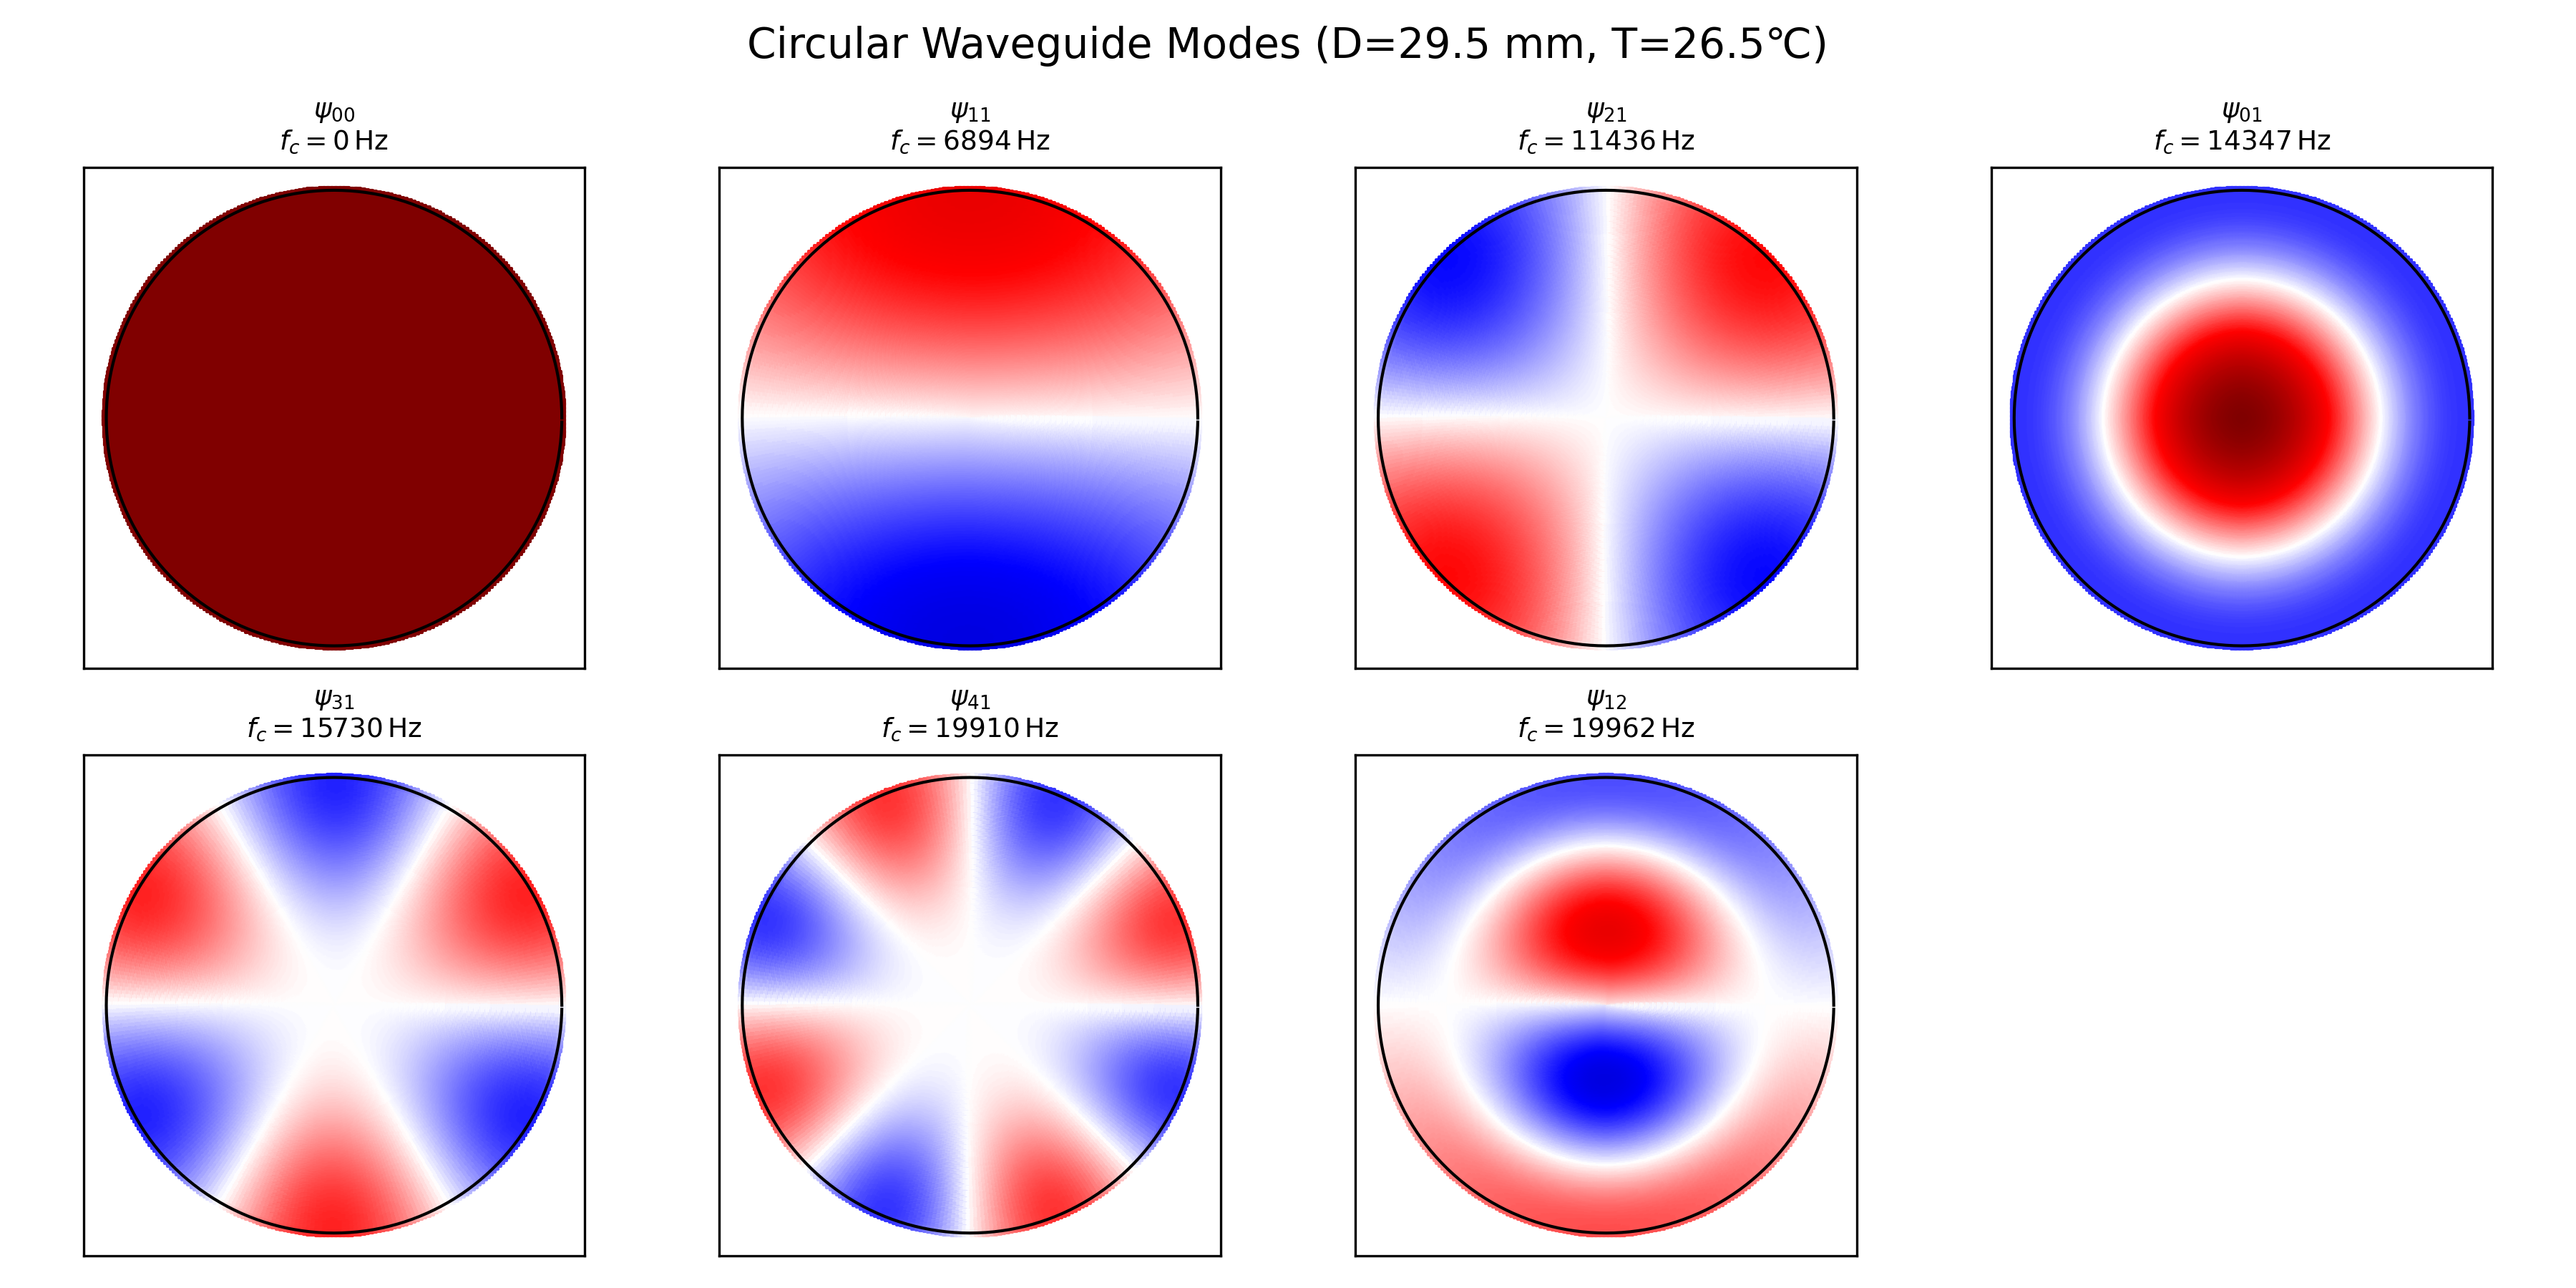
\includegraphics[width=0.9\textwidth]{../02-code/circle_modes.png}
    \caption{Python 生成的圆管模态形状($D=29.5$ mm,$T=26.5^{\circ}$C)。灰度表示声压相位;黑线为零幅节点。}
    \label{fig:circ-modes}
\end{figure}

\paragraph{幅值差异的物理原因} 图中两条曲线的幅度相差可达几十分贝,这是因为本例\emph{传递函数的定义}取的是端面\textbf{平均声压之比} $H(f)=\bar P(z=L)/\bar P(z=0)$,且采用"左端单位体积流速源 + 左端硬壁"激励。在这样的驱动方式下:
\begin{itemize}
  \item 当右端同为硬壁 (Hard--Hard) 时,单位流量无法排出,两端形成压力腹\,/\,腹驻波,右端平均压强随共振堆积,可达很高幅值;
  \item 当右端为零压力 (Hard--Zero) 时,右端压强被钳制为零,同一单位流源只能在管内建立较低压强,因而 $|H|$ 整体显著降低。
\end{itemize}
因此幅度差大并非计算错误,而是两种边界对"右端平均压强"的物理响应截然不同。如果更关注共振频率而非幅值大小,可改用"左端零压激励"或直接比较阻抗谱。

%======================================================================
\section{结论与展望}
%======================================================================

\begin{enumerate}
    \item \textbf{理论门槛}:圆管 $(1,1)$ 模态截止频率与半径成反比;例如 $R\approx\SI{2}{\centi\meter}$ ($D\approx\SI{4}{\centi\meter}$) 时 $f_c\approx\SI{5}{\kilo\hertz}$,而 $R\approx\SI{1}{\centi\meter}$ 时 $f_c\approx\SI{10}{\kilo\hertz}$。对于本文关注的 $D=\SI{29.5}{mm}$ ($R=\SI{14.75}{mm}$) 波导,首个高阶模态 $(\psi_{11})$ 的截止频率精确计算为 \SI{6.9}{kHz}。
    \item \textbf{实际声道}:喉道最窄处可低至 \SI{0.5}{\centi\meter} \textasciitilde{} \SI{1}{\centi\meter}(对应 $f_c\gtrsim\SI{10}{\kilo\hertz}$ 至 \SI{20}{\kilo\hertz}),而口腔后部可达 \SI{4}{\centi\meter}$\,$($f_c\approx\SI{5}{\kilo\hertz}$)。这表明在声道不同位置,高阶模态出现的起始频率是不同的。
    \item \textbf{物理后果}:当频率超过相应截止频率后,截面声压不再均匀,一维面积函数模型失效;需采用多模态/三维数值方法(FEM、FDM、BEM 等)研究高频行为。
\end{enumerate}

总结来说:
\begin{itemize}
    \item 对于直径 $D=\SI{29.5}{mm}$ 的理想圆柱波导,在约 \SI{6.9}{kHz} 以下,平面波模型是声场的一个良好近似。
    \item 当频率高于 \SI{6.9}{kHz},$\psi_{11}$ 及其后更高阶的横向模态可以传播,此时必须使用三维或多模态方法才能准确描述声场。
    \item 尽管实际声道几何形状复杂多变,导致三维效应出现的具体频率难以一概而论,但对于类似尺寸的管状结构,\SI{6.9}{kHz} (或工程上更保守的如 \SI{5}{\kilo\hertz} 至 \SI{7}{\kilo\hertz}) 可以视为一个重要的参考分界点,提示研究者关注高频下平面波假设的局限性。
\end{itemize}
未来的工作可以拓展到更接近实际声道的变截面、弯曲波导,并考虑粘滞热损耗对高阶模态传播特性的影响。

%======================================================================
\section{参考公式速查}
%======================================================================

\[
    \boxed{\lambda = \dfrac{c}{f}}, \qquad
    \boxed{f_{c,mn} = \dfrac{c}{2\pi}\dfrac{\mu_{mn}}{R}}, \qquad
    \boxed{\mu_{11}\approx1.841}.
\]

%======================================================================
\section{参考文献}
%======================================================================

\begin{enumerate}
    \item P.\,M.~Morse \& K.\,U.~Ingard, \emph{Theoretical Acoustics}, Princeton Univ.\ Press, 1968.
    \item N.\,H.~Fletcher \& T.\,D.~Rossing, \emph{The Physics of Musical Instruments}, Springer, 1998.
    \item B.\,B.~Monson \emph{et~al.}, ``Auditory processing of high-frequency energy…'', \emph{JASA}, 2014.
\end{enumerate}

%======================================================================
\section{有限长圆管传递函数示例}
\label{sec:tube_tf}
%======================================================================

在前文推导了圆柱波导高阶模态的截止频率之后,本节给出一个\textbf{有限长}圆管在一维平面波假设下的传递函数数值示例,并比较两种端面边界:

\begin{itemize}
  \item 左端 \textbf{硬壁 (Hard)},右端 \textbf{硬壁 (Hard)};
  \item 左端 \textbf{硬壁 (Hard)},右端 \textbf{零压力 (Zero)}。
\end{itemize}

参数取直径 $D=\SI{29.5}{mm}$、长度 $L=\SI{15}{cm}$、温度 $T=\SI{26.5}{\celsius}$,频率范围 $1\,\mathrm{Hz}\,\text{--}\,10\,\mathrm{kHz}$。计算脚本位于 
\texttt{helper/02-code/tube\_transfer\_compare.py},运行后会自动生成比较图 \texttt{tube\_transfer\_compare.png}(同时导出 PDF)。

图~\ref{fig:tube-tf-compare} 显示了幅度与相位随频率变化的对比。可以看到:

\begin{itemize}
  \item 双硬壁管道在 $f=\tfrac{pc}{2L}$ ($p=1,2,\dots$) 处呈现压力腹共振(幅值峰值),其间隔约 \SI{1.15}{kHz};
  \item 硬壁--零压组合则在 $f=\tfrac{(2p+1)c}{4L}$ 出现共振,频率上移四分之一波长,幅度模式亦不同;
  \item 两种边界在低频 (\SI{<500}{Hz}) 传递函数几乎重合,验证了平面波模型与端面反射相位差的物理解释。
\end{itemize}

\begin{figure}[h]
    \centering
    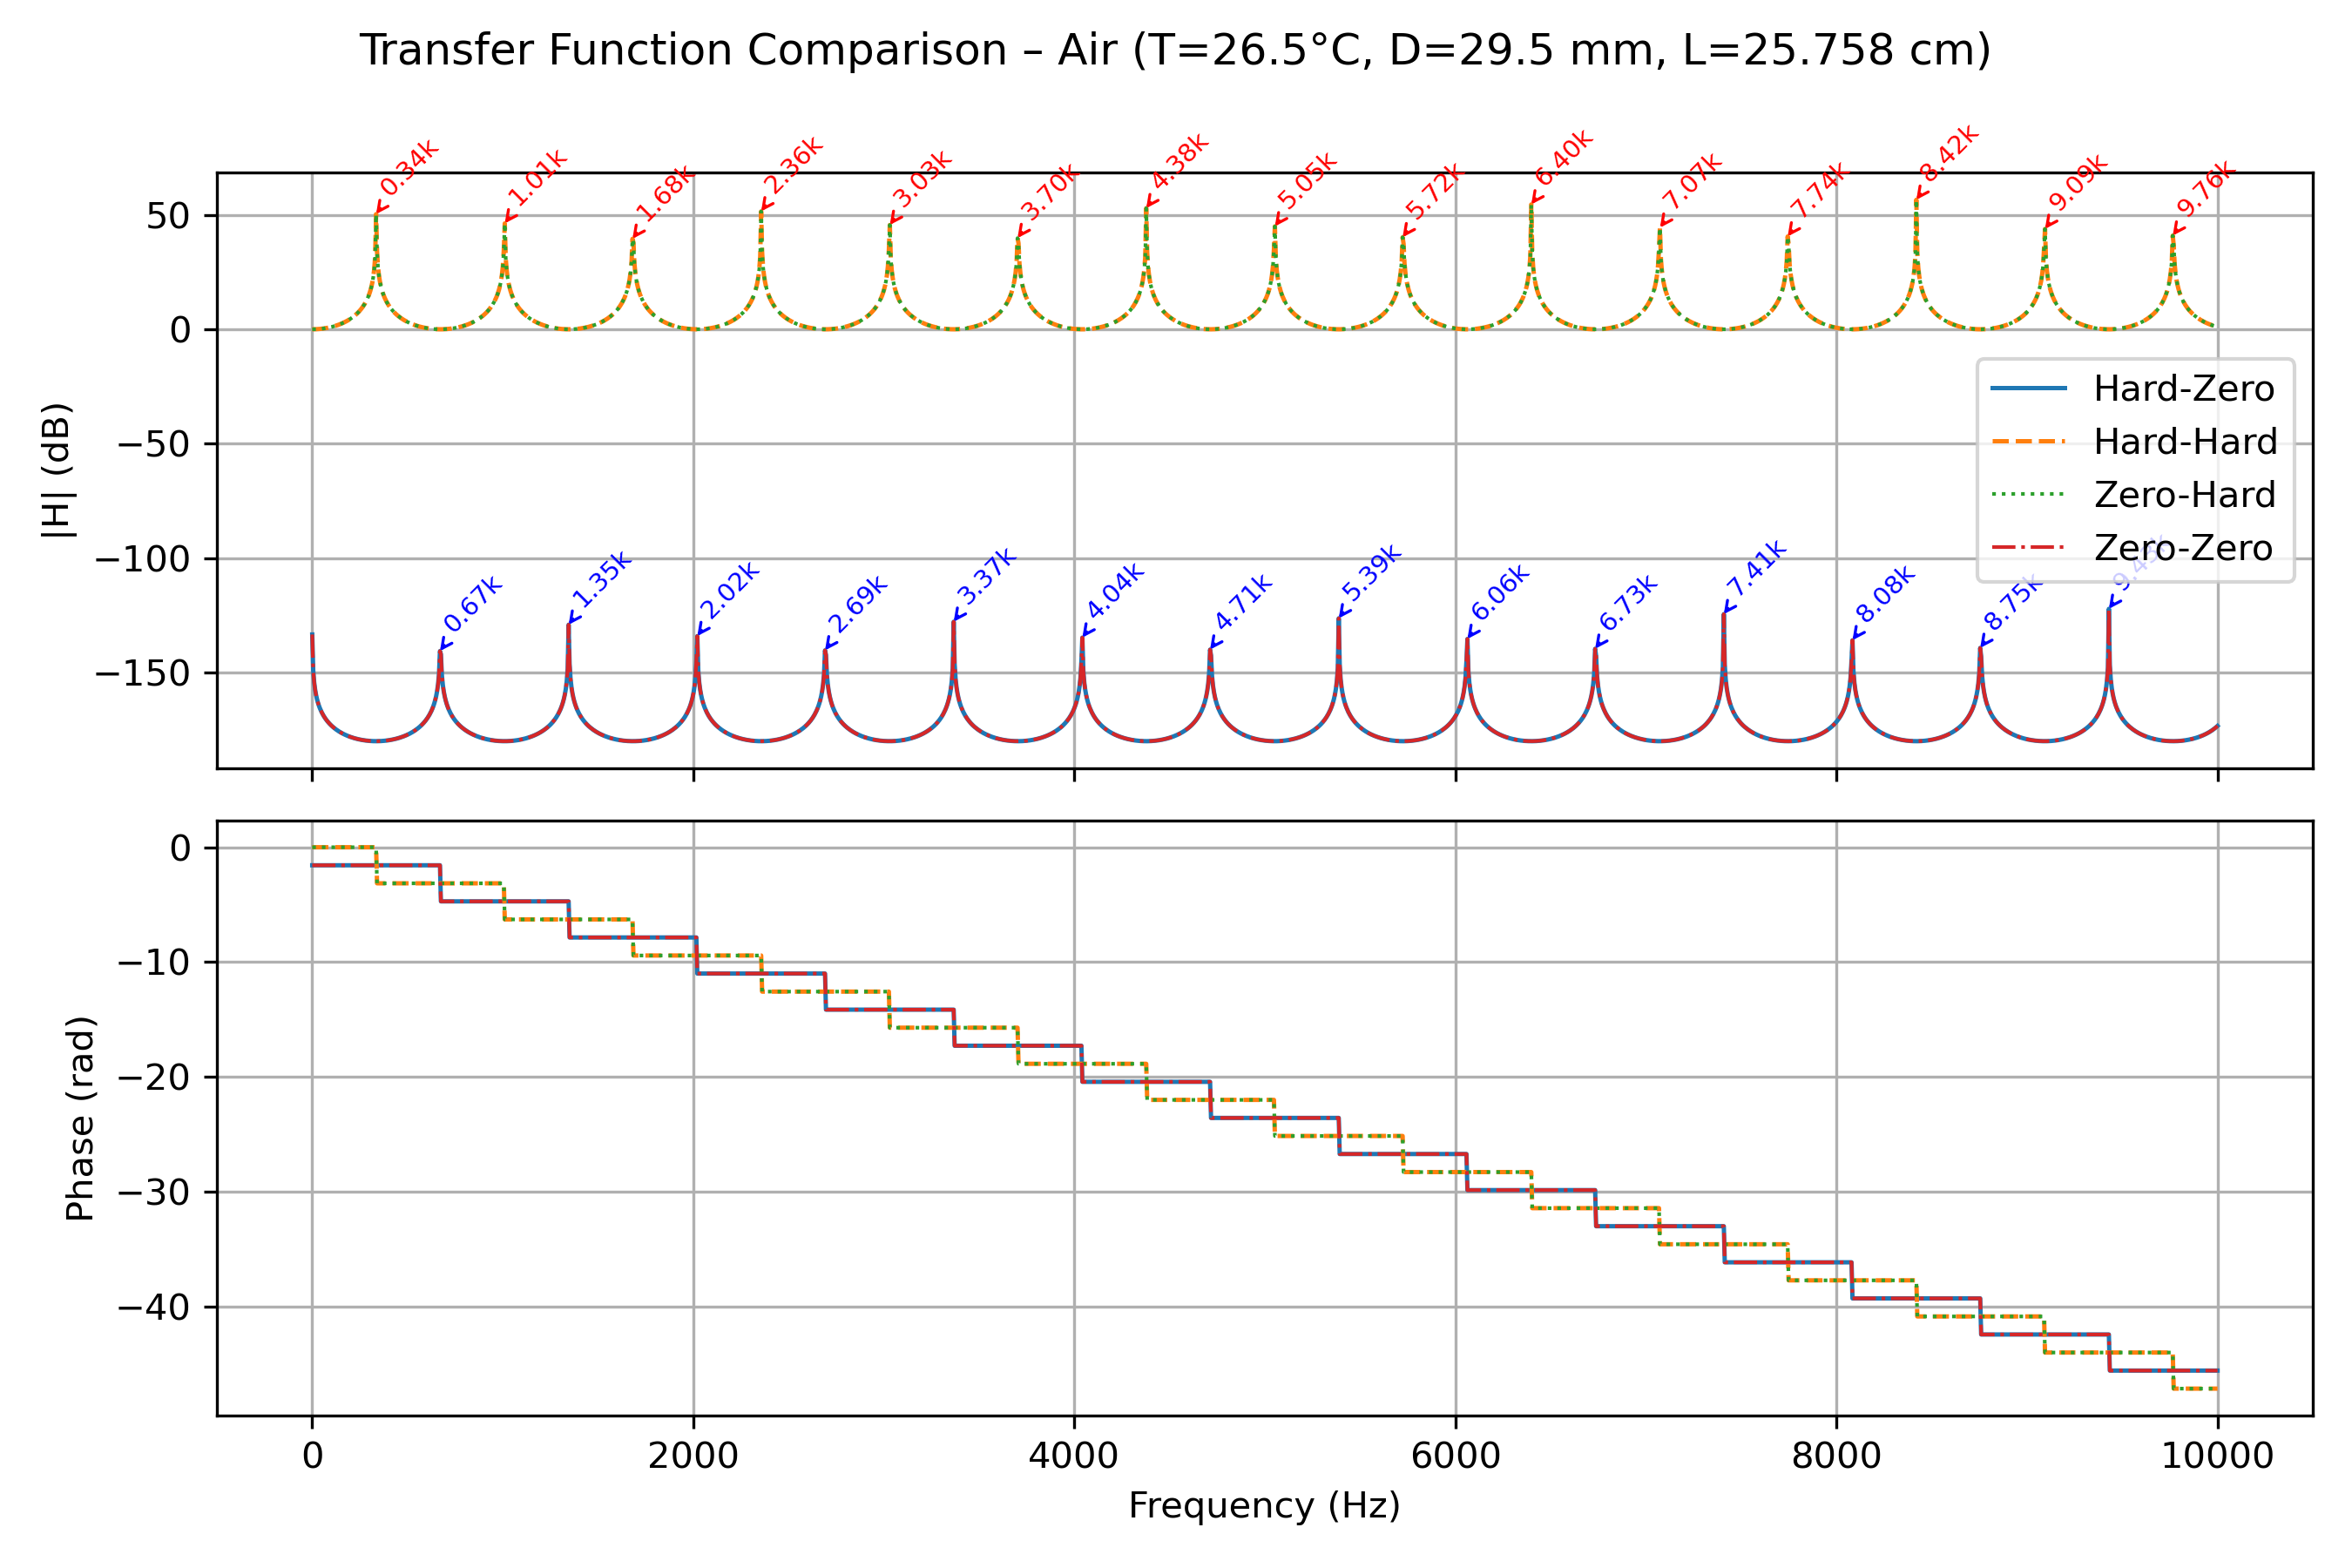
\includegraphics[width=0.98\textwidth]{../02-code/tube_transfer_compare.png}
    \caption{有限长圆管 ($D=\SI{29.5}{mm},\,L=\SI{15}{cm}$) 传递函数幅度与相位:硬壁--硬壁 vs. 硬壁--零压}
    \label{fig:tube-tf-compare}
\end{figure}

以上结果进一步验证了边界条件对声管共振特性的决定作用,也为之后引入高阶模态/辐射阻抗提供了参考基线。

\end{document}
